\documentclass[journal,12pt,twocolumn]{IEEEtran}
\usepackage{setspace}
\usepackage{gensymb}
\usepackage{xcolor}
\usepackage{caption}
\singlespacing
\usepackage{siunitx}
\usepackage[cmex10]{amsmath}
\usepackage{mathtools}
\usepackage{hyperref}
\usepackage{amsthm}
\usepackage{mathrsfs}
\usepackage{txfonts}
\usepackage{stfloats}
\usepackage{cite}
\usepackage{cases}
\usepackage{subfig}
\usepackage{longtable}
\usepackage{multirow}
\usepackage{enumitem}
\usepackage{bm}
\usepackage{mathtools}
\usepackage{listings}
\usepackage{tikz}
\usetikzlibrary{shapes,arrows,positioning}
\usepackage{circuitikz}
\renewcommand{\vec}[1]{\boldsymbol{\mathbf{#1}}}
\DeclareMathOperator*{\Res}{Res}
\renewcommand\thesection{\arabic{section}}
\renewcommand\thesubsection{\thesection.\arabic{subsection}}
\renewcommand\thesubsubsection{\thesubsection.\arabic{subsubsection}}

\renewcommand\thesectiondis{\arabic{section}}
\renewcommand\thesubsectiondis{\thesectiondis.\arabic{subsection}}
\renewcommand\thesubsubsectiondis{\thesubsectiondis.\arabic{subsubsection}}
\hyphenation{op-tical net-works semi-conduc-tor}

\lstset{
language=Python,
frame=single, 
breaklines=true,
columns=fullflexible
}
\begin{document}
\theoremstyle{definition}
\newtheorem{theorem}{Theorem}[section]
\newtheorem{problem}{Problem}
\newtheorem{proposition}{Proposition}[section]
\newtheorem{lemma}{Lemma}[section]
\newtheorem{corollary}[theorem]{Corollary}
\newtheorem{example}{Example}[section]
\newtheorem{definition}{Definition}[section]
\newcommand{\BEQA}{\begin{eqnarray}}
\newcommand{\EEQA}{\end{eqnarray}}
\newcommand{\define}{\stackrel{\triangle}{=}}
\newcommand{\myvec}[1]{\ensuremath{\begin{pmatrix}#1\end{pmatrix}}}
\newcommand{\mydet}[1]{\ensuremath{\begin{vmatrix}#1\end{vmatrix}}}
\bibliographystyle{IEEEtran}
\providecommand{\nCr}[2]{\,^{#1}C_{#2}} % nCr
\providecommand{\nPr}[2]{\,^{#1}P_{#2}} % nPr
\providecommand{\mbf}{\mathbf}
\providecommand{\pr}[1]{\ensuremath{\Pr\left(#1\right)}}
\providecommand{\qfunc}[1]{\ensuremath{Q\left(#1\right)}}
\providecommand{\sbrak}[1]{\ensuremath{{}\left[#1\right]}}
\providecommand{\lsbrak}[1]{\ensuremath{{}\left[#1\right.}}
\providecommand{\rsbrak}[1]{\ensuremath{{}\left.#1\right]}}
\providecommand{\brak}[1]{\ensuremath{\left(#1\right)}}
\providecommand{\lbrak}[1]{\ensuremath{\left(#1\right.}}
\providecommand{\rbrak}[1]{\ensuremath{\left.#1\right)}}
\providecommand{\cbrak}[1]{\ensuremath{\left\{#1\right\}}}
\providecommand{\lcbrak}[1]{\ensuremath{\left\{#1\right.}}
\providecommand{\rcbrak}[1]{\ensuremath{\left.#1\right\}}}
\theoremstyle{remark}
\newtheorem{rem}{Remark}
\newcommand{\sgn}{\mathop{\mathrm{sgn}}}
\newcommand{\rect}{\mathop{\mathrm{rect}}}
\newcommand{\sinc}{\mathop{\mathrm{sinc}}}
\providecommand{\abs}[1]{\left\vert#1\right\vert}
\providecommand{\res}[1]{\Res\displaylimits_{#1}} 
\providecommand{\norm}[1]{\left\Vert#1\right\Vert}
\providecommand{\mtx}[1]{\mathbf{#1}}
\providecommand{\mean}[1]{E\left[ #1 \right]}
\providecommand{\fourier}{\overset{\mathcal{F}}{ \rightleftharpoons}}
\providecommand{\ztrans}{\overset{\mathcal{Z}}{ \rightleftharpoons}}
\providecommand{\system}[1]{\overset{\mathcal{#1}}{ \longleftrightarrow}}
\newcommand{\solution}{\noindent \textbf{Solution: }}
\providecommand{\dec}[2]{\ensuremath{\overset{#1}{\underset{#2}{\gtrless}}}}
\let\StandardTheFigure\thefigure
\def\putbox#1#2#3{\makebox[0in][l]{\makebox[#1][l]{}\raisebox{\baselineskip}[0in][0in]{\raisebox{#2}[0in][0in]{#3}}}}
     \def\rightbox#1{\makebox[0in][r]{#1}}
     \def\centbox#1{\makebox[0in]{#1}}
     \def\topbox#1{\raisebox{-\baselineskip}[0in][0in]{#1}}
     \def\midbox#1{\raisebox{-0.5\baselineskip}[0in][0in]{#1}}

\vspace{3cm}
\title{Circle Assignment}
\author{Gautam Singh}
\maketitle
\bigskip

\begin{abstract}
    This document contains the solution to Question 6 of 
    Exercise 4 in Chapter 10 of the class 9 NCERT textbook.
\end{abstract}

\begin{enumerate}
    \item A circular park of radius 20 m is situated in a colony. Three boys 
    Ankur, Syed and David are sitting at equal distance on its boundary each 
    having a toy telephone in his hands to talk each other. Find the length of 
    the string of each phone.

    \solution Let the position vectors of the boys be
    \begin{align}
        \vec{A} = \myvec{r\\0},\ \vec{S} = \myvec{r\cos\beta\\r\sin\beta},\ \vec{D} = \myvec{r\cos\gamma\\r\sin\gamma}
        \label{eq:pos-vec-def}
    \end{align}
    where
    \begin{align}
        \beta, \gamma \in [0,2\pi),\ \beta, \gamma \neq 0
        \label{eq:int}
    \end{align}
    We have,
    \begin{align}
        \norm{\vec{A}-\vec{S}}^2 &= \norm{\vec{A}-\vec{D}}^2 \\
        \implies \vec{A}^\top\vec{S} &= \vec{A}^\top\vec{D} \\
        \implies \cos\beta &= \cos\gamma \\
        \implies \sin\frac{\beta+\gamma}{2}\sin\frac{\beta-\gamma}{2} &= 0
    \end{align}
    Since $\beta \neq \gamma$ and from \eqref{eq:int}, 
    $\frac{\beta-\gamma}{2} \in \brak{-\pi,\pi}$, we get that
    \begin{align}
        \frac{\beta+\gamma}{2} &= n\pi \\
        \implies \beta+\gamma &= 2n\pi
        \label{eq:sum}
    \end{align}
    However, \eqref{eq:int} gives $\beta + \gamma \in \brak{0,4\pi}$, which forces
    $n = 1$ in \eqref{eq:sum}, and thus
    \begin{align}
        \beta + \gamma = 2\pi
        \label{eq:bg-sum}
    \end{align}
    Therefore, using \eqref{eq:bg-sum}
    \begin{align}
        &\norm{\vec{A}-\vec{S}}^2 = \norm{\vec{S}-\vec{D}}^2 \\
        &\implies \vec{A}^\top\vec{S} = \vec{D}^\top\vec{S} \\
        &\implies \cos\beta = \cos\brak{\beta-\gamma} \\
        &\implies \sin\frac{3\beta-2\pi}{2}\sin\frac{\gamma}{2} = 0
        \label{eq:beta-gamma}
    \end{align}
    From \eqref{eq:beta-gamma} and \eqref{eq:int},
    \begin{align}
        3\beta -2\pi &= 2m\pi \\
        \implies 3\beta &= 2k\pi \\
        \implies \beta &= \frac{2k\pi}{3}
    \end{align}
    where $k \in \mathbb{Z}$. From \eqref{eq:int}, $k \in \cbrak{1,2}$.
    Thus,
    \begin{align}
        \beta,\gamma \in \cbrak{\frac{2\pi}{3},\frac{4\pi}{3}}
        \label{eq:bg-sol}
    \end{align}
    Therefore, the length of the thread from \eqref{eq:bg-sol} is
    \begin{align}
        \norm{\vec{S}-\vec{D}} &= \norm{r\myvec{\cos\beta-\cos\gamma\\\sin\beta-\sin\gamma}} \\
                               &= r\sqrt{3}
    \end{align}
    Here, $r = 20$ m. Thus, the length is $20\sqrt{3}$ m.

    The situation is demonstrated in Fig. \ref{fig:equilateral}, plotted by the 
    Python code \texttt{codes/equilateral.py}. Here, the values used for 
    construction are shown in Table \eqref{tab:param}.
    \begin{table}[!ht]
        \centering
        \begin{tabular}{|c|c|}
            \hline
            \textbf{Parameter} & \textbf{Value} \\
            \hline
            $r$ & 20 \\
            \hline
            $\beta$ & $\frac{2\pi}{3}$ \\
            \hline
            $\gamma$ & $\frac{4\pi}{3}$ \\
            \hline
        \end{tabular}
        \caption{Parameters used in the construction of Fig. \ref{fig:equilateral}.}
        \label{tab:param}
    \end{table}
    \begin{figure}[!ht]
        \centering
        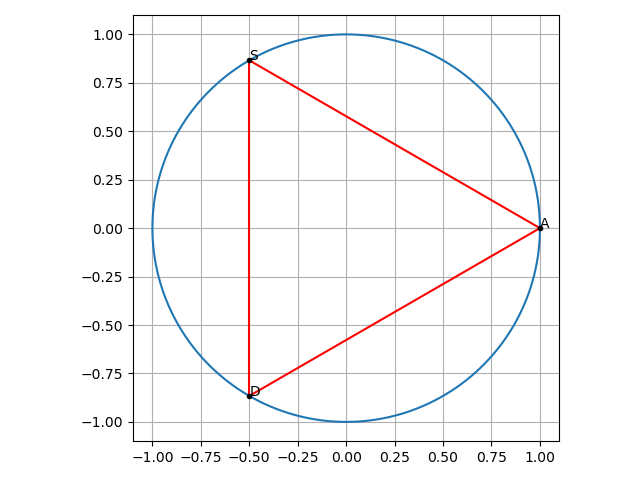
\includegraphics[width=\columnwidth]{figs/equilateral.png}
        \caption{$ASD$ is an equilateral triangle of side $20\sqrt{3}$ m.}
        \label{fig:equilateral}
    \end{figure}
\end{enumerate}
\end{document}
